\section{Базовый алгоритм}
Базовым алгоритмом в данной задаче является PLS \cite{Haenlein2004}. Для проведения эксперимента, из данных электрокортикограммы были выделены частоты сигналов, в соответствие которым были поставлены трехмерные координаты движения руки обезьяны. Полученные данные были разделены на обучающую и контрульную выборки. Результаты эксперемента представлены на рисунке \ref{fig:baseAlgo}.
\begin{figure}
  \begin{center}
    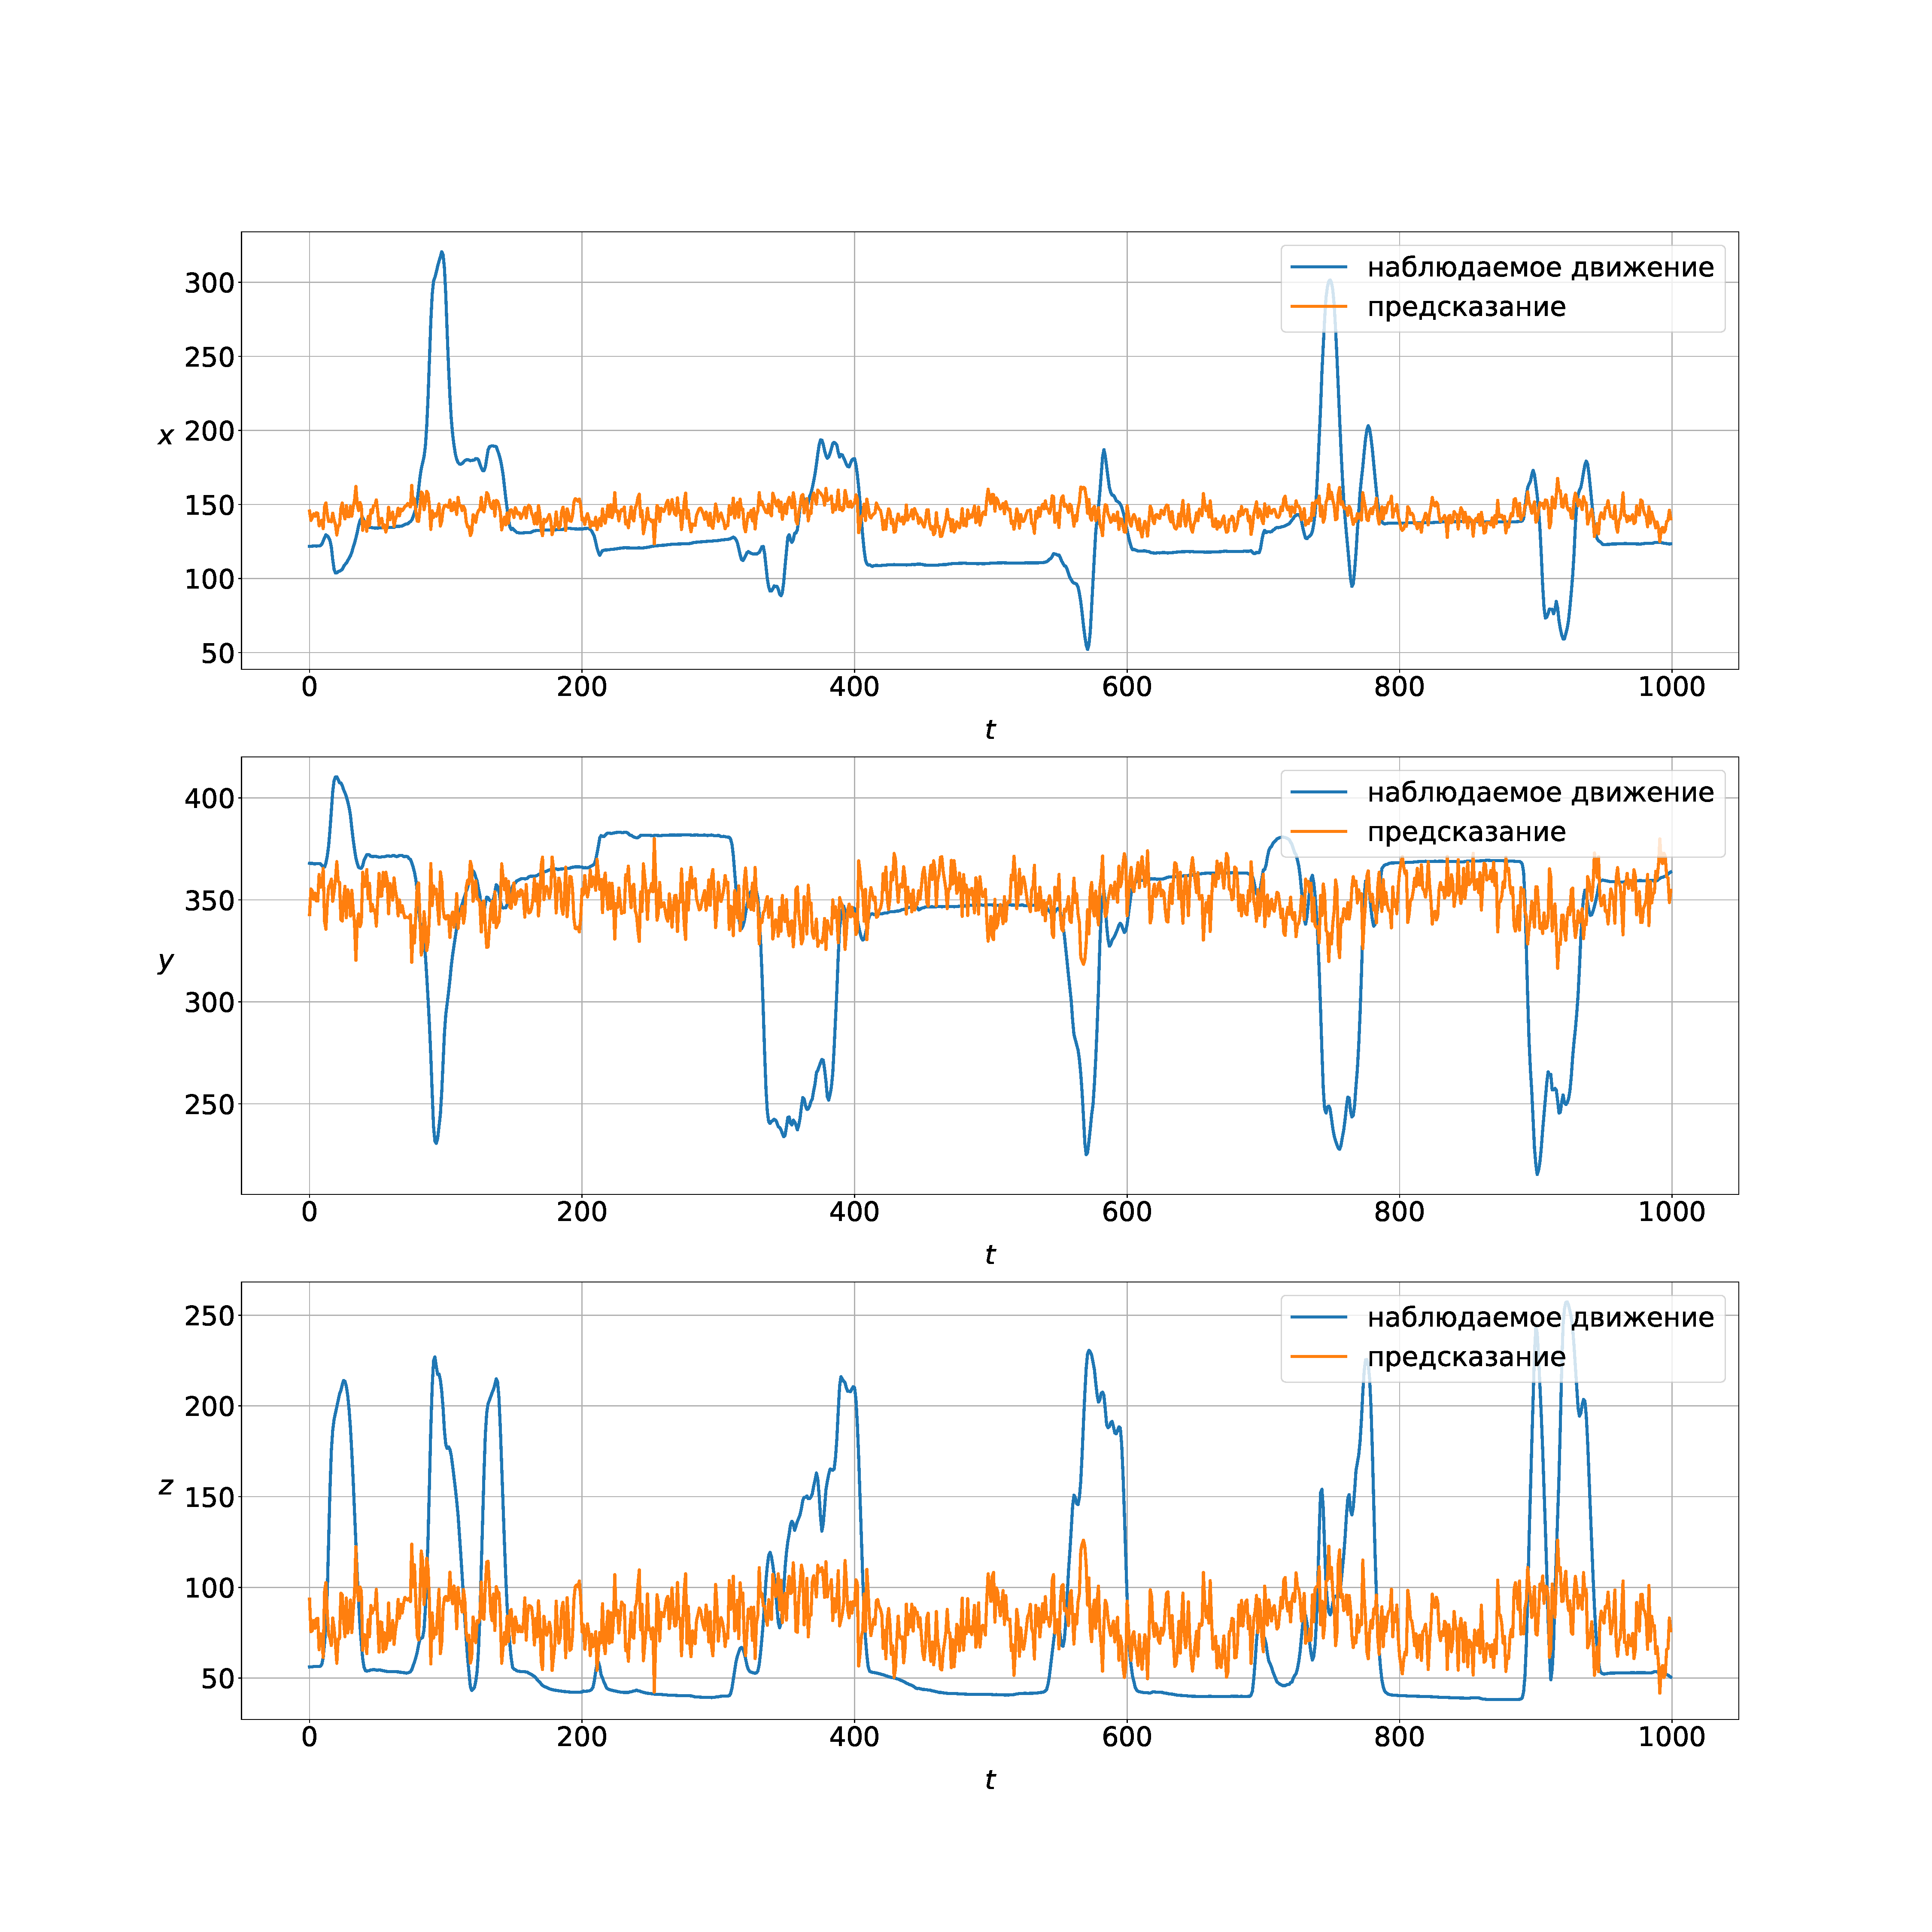
\includegraphics[width=\textwidth]{pls.pdf}
    \caption{Результаты эксперимента с базовым алгоритмом}
    \label{fig:baseAlgo}
  \end{center}
\end{figure}
На графике представлена зависимость координаты конечности от времени. Как видно из рисунка, базовый алгоритм довольно плохо справляется с поставленной задачей. Несмотря на то, что общий профиль пиков соблюдается, PLS не предсказывает острые пики, а также предсказывает флуктуации координаты во время, когда конечность почти не движется. В результате погрешность предсказания высока. Для борьбы с этим предлагается уменьшать размерность задачи, а значит и связанность данных.
